\documentclass{beamer}
\usepackage{multicol}
\usepackage{bm}
\usepackage{prooftree}
\setlength{\columnsep}{0.5cm}

\mode<presentation>
    {
      \usetheme{Frankfurt}
      \usecolortheme{default}
      \usefonttheme{default}
      \setbeamertemplate{footline}[frame number]
      \setbeamertemplate{navigation symbols}{}
    }

    \usepackage[english]{babel}
    \usepackage[utf8x]{inputenc}
    \title[Audition]{Tactique automatique en Coq}

    \author{Quentin Garchery}
    \date{Lundi 26 novembre 2018}

    \begin{document}

    \begin{frame}
      \begin{center}
        \maketitle
        \normalsize{LRI, Paris-Saclay\\
          Univ. Paris-Sud / Inria }
        \vspace{1mm}


        \vspace{1mm}

        \begin{multicols}{2}
          \normalsize Chantal Keller \\
          \scriptsize LRI, Univ. Paris-Sud \\

          \normalsize Valentin Blot \\
          \scriptsize IRIF, Univ. Paris 7
        \end{multicols}

      \end{center}
    \end{frame}



    \section{Introduction}

    \subsection{}
    \begin{frame}{Vue d'ensemble}


      Les logiciels formels permettent de vérifier des propriétés mathématiques. On considère deux types de logiciels formels :
      \begin{itemize}
      \item Assistants de preuve, expressifs et interactifs
      \item Prouveurs automatiques de type SMT, moins expressifs mais l'effort de certification est plus restreint

      \end{itemize}

      \vspace{0.5cm}
      Cadre : communication entre ces deux types de logiciels pour bénéficier de leurs avantages respectifs.

    \end{frame}


    \subsection{}
    \begin{frame}{Automatisation dans les assistants de preuve}
      Deux approches à l'intégration d'un prouveur automatique dans un assistant de preuve :
      \begin{multicols}{2}
        \begin{center}
          \textit{Approche autarcique}
        \end{center}
        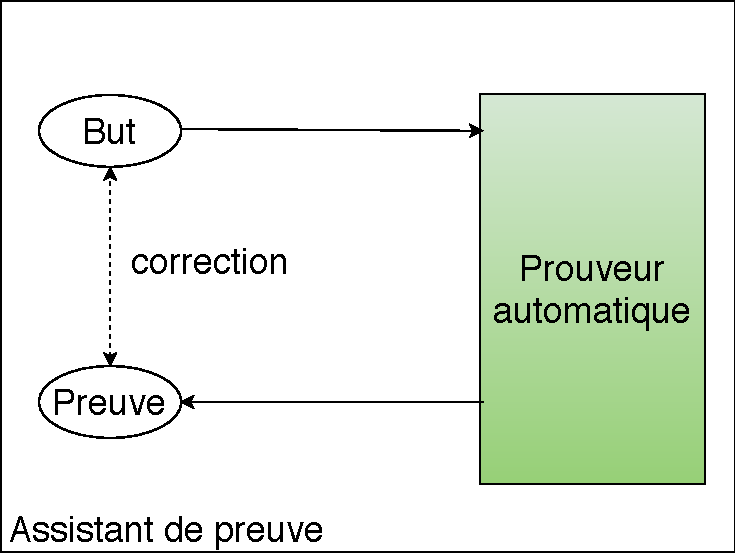
\includegraphics[height=3.8cm]{1_Autarcique.pdf}\\
        Vérifier le code du prouveur automatique. \\
        \begin{center}
          \textit{Approche sceptique}
        \end{center}
        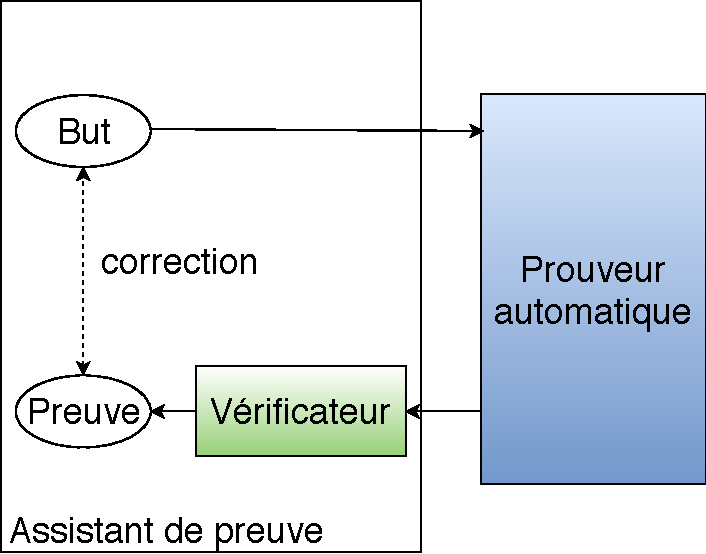
\includegraphics[height=3.8cm]{2_Sceptique.pdf}\\
        Vérifier la réponse du prouveur automatique.
      \end{multicols}
    \end{frame}



    \section{SMTCoq}

    \subsection{}
    \begin{frame}{Présentation de SMTCoq}
      SMTCoq est une interface entre Coq et différents prouveurs automatiques (veriT, CVC4) qui est actuellement développée par Chantal Keller et Valentin Blot en collaboration avec l'Université de l'Iowa. \\
      \vspace*{3mm}
      But : amélioration de l'automatisation de Coq et de la confiance dans les prouveurs automatiques. \\
      \vspace*{3mm}
      Permet de prouver automatiquement le théorème suivant :
      \[ \forall x \forall y \forall f. x \neq y + 1 \vee f(y) = f(x-1) \]
      Fragment supporté : logique propositionnelle, arithmétique linéaire sur $\mathbb{Z}$, égalité et fonctions non-interprétées, théorie des tableaux, théorie des vecteurs de bit, variables quantifiées universellement en tête de formule.

    \end{frame}




    \subsection{}
    \begin{frame}{SMTCoq en détail : approche sceptique}

      \begin{center}
        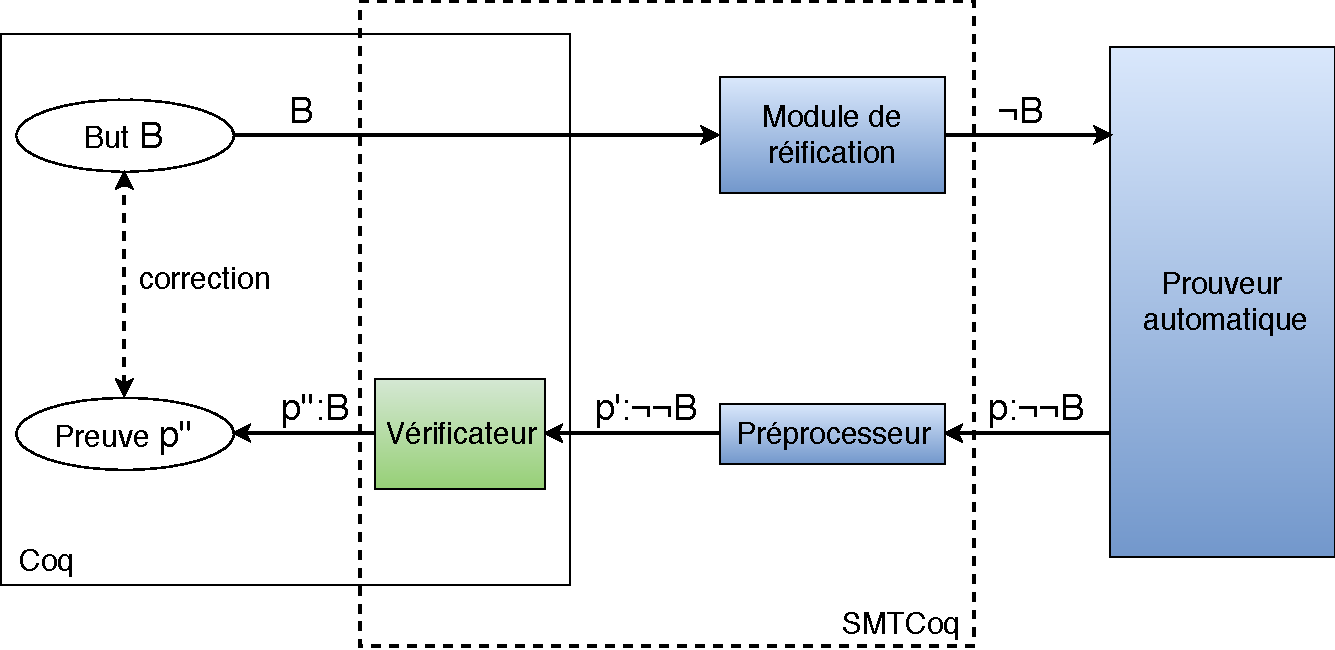
\includegraphics[height=5cm]{smt_auto.pdf}
      \end{center}

      En transmettant la négation du but au prouveur automatique, on obtient un certificat prouvant l'absurde. Dans les cas d'application de SMTCoq, la double négation du but implique le but.


    \end{frame}

    \subsection{}
    \begin{frame}{Définitions et preuves en Coq}

      La structure de données des formules de SMTCoq est définie par un type inductif :

      \texttt{Inductive formula := }\\
      \texttt{| Bool (b\,:\,bool)}\\
      \texttt{| And (f1\,:\,formula) (f2\,:\,formula).}

      \vspace{0.5cm}
      L'interprétation calcule la valeur d'une formule de SMTCoq :
      \texttt{Fixpoint interp t := match t with}\\
      \texttt{| Bool b => b}\\
      \texttt{| And f1 f2 => interp f1 \&\& interp f2.}

      \vspace{0.5cm}
      Un lemme prouvable :

      \texttt{Lemma andproj1 f1 f2 : }\\
      \texttt{  interp (And f1 f2) = true -> interp f1 = true.}


    \end{frame}

    \subsection{}
    \begin{frame}{Réification}

      La réification du terme  \texttt{(true\,\&\&\,false)\,\&\&\,(false\,\&\&\,true)}
      est donnée par
      \begin{align*}
        \texttt{And }  &\texttt{(And (Bool true) (Bool false))}\\
        &\texttt{(And (Bool false) (Bool true))}
      \end{align*}
      qui représente l'arbre suivant :
      \begin{center}
        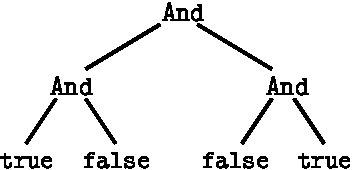
\includegraphics[height=2.2cm]{booltree.pdf}
      \end{center}

      Réification : rendre explicite la structure d'un terme en l'exprimant dans une structure de données.


      \vspace{2mm}

      Dans le cas de SMTCoq, cela permet entre autres l'écriture du problème dans un fichier servant d'entrée aux prouveurs.
    \end{frame}

    \subsection{}
    \begin{frame}{SMTCoq en détail}

      \begin{center}
        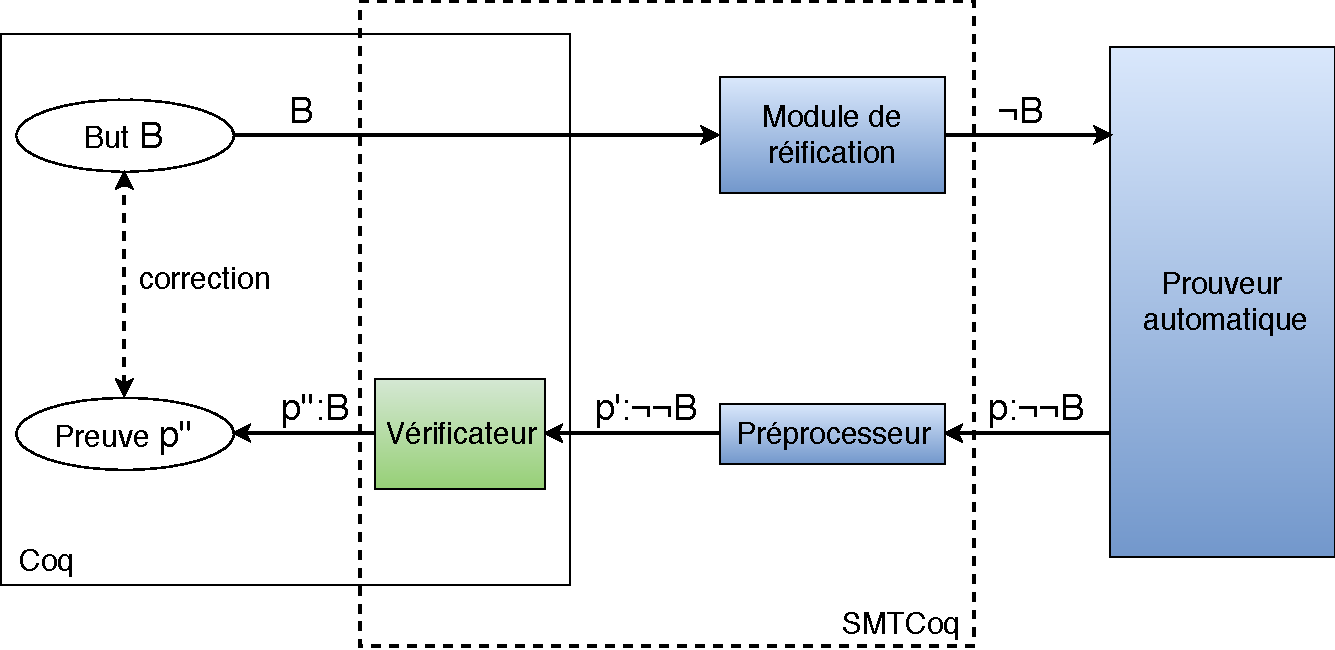
\includegraphics[height=5cm]{smt_auto.pdf}
      \end{center}


    \end{frame}

    \subsection{}
    \begin{frame}{Préprocesseur}
      Le préprocesseur de SMTCoq remplit plusieurs objectifs :
      \begin{itemize}
      \item \textbf{parsing} des fichiers de certificats en un type de données OCaml
      \item \textbf{adaptations} des certificats, celles-ci sont par exemple nécessaires lorsque la logique du prouveur automatique diffère de celle de Coq
      \item \textbf{simplifications} en regroupant les règles du certificat au fonctionnement similaire
      \item \textbf{optimisations} des certificats, par exemple en élaguant les règles redondantes
      \end{itemize}
    \end{frame}

    \subsection{}
    \begin{frame}{SMTCoq en détail}

      \begin{center}
        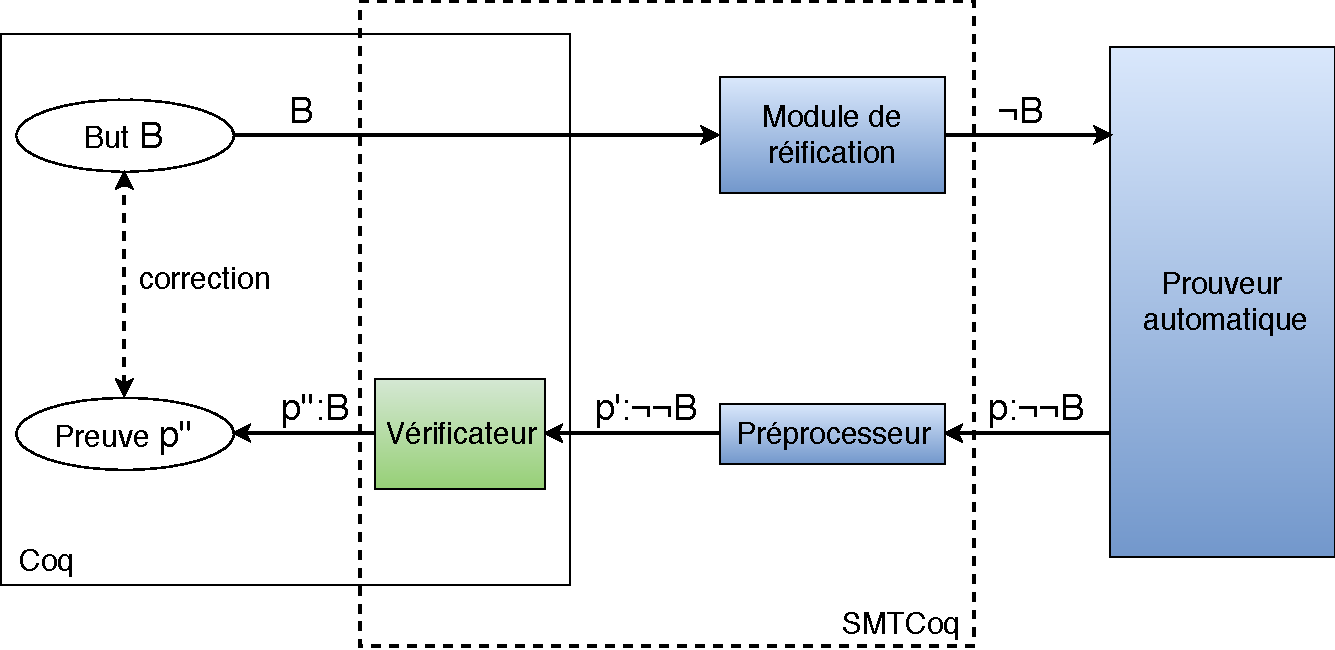
\includegraphics[height=5cm]{smt_auto.pdf}
      \end{center}


    \end{frame}

    \subsection{}
    \begin{frame}{Vérificateur : les règles et les certificats}

      \texttt{Inductive rule :=}\\
      \texttt{| AndProj (pos\_prem\,:\,int) (ind\_proj\,:\,int)}\\
      \texttt{| Resolution (pos\_param\,:\,int list)}.


      \vspace{0.5cm}

      Une règle \texttt{Andproj prem i} permet de projeter la conjonction en indice \texttt{prem} sur sa composante \texttt{i}.

      \vspace{0.5cm}

      Le certificat Coq est obtenu à partir du fichier de certificat fourni par les prouveurs automatiques.
    \end{frame}

    \begin{frame}{Vérificateur : la fonction \textit{checker}}

      La fonction \texttt{checker} prend en argument un certificat et une formule et maintient une liste de formules appelé \textit{état}.

      \vspace {0.3cm}

      Posons : \\
      \texttt{certif := [Andproj 0 2; Andproj 0 1; Resolution 2 1]}\\
      \texttt{in := And (Bool x) (Neg (Bool x))}\\
      \vspace{0.3cm}
      \uncover<1->{L'état est alors initialisé à \texttt{[in]}.}

      \vspace{1mm}
      \uncover<1->{Après la première règle : \texttt{[in; Bool x]}. }

      \vspace{1mm}
      \uncover<2->{Après la deuxième règle : \texttt{[in; Bool x; Neg (Bool x)]}. }

      \vspace{1mm}
      \uncover<3->{Enfin, la troisième règle transforme l'état en :
        \[\texttt{[in; Bool x; Neg (Bool x); Bool false]}\]

        L'état final contient \texttt{Bool false}, on a donc :
        \[\texttt{checker certif in = true}\]
      }
    \end{frame}


    \begin{frame}{Vérificateur : le théorème de correction}

      \begin{block}{ Théorème de correction}
        Si \texttt{checker certif in = true} pour un certificat \texttt{certif} et une formule d'entrée \texttt{in} alors \texttt{in} n'est pas satisfiable.
      \end{block}

      \textit{Point clé de la preuve} : le lemme de correction d'une étape.\\
      Ce lemme nous assure que chaque règle ajoute à l'état une nouvelle formule vraie dans l'état courant.


      \vspace{2mm}

      Pour rétablir la preuve de correction lorsqu'on ajoute un nouveau type de règle, il suffit de compléter ce lemme pour ce nouveau type.

      \vspace{2mm}

      \begin{prooftree}
        \AxiomC{}
        \RightLabel{\textit{refl}}
        \UnaryInfC{\texttt{true = true}}
        \RightLabel{\textit{conv}}
        \UnaryInfC{\texttt{checker certif in = true}}
        \AxiomC{\textit{correction d'une étape}}
        \UnaryInfC{\textit{correction}}
        \RightLabel{\textit{MP}}
        \BinaryInfC{\texttt{interp in = false}}
      \end{prooftree}

      L'hypothèse du théorème de correction est obtenue en lançant le calcul de la fonction \texttt{checker}, c'est la réflexion calculatoire.


    \end{frame}





    \section{Ajout de lemmes quantifiés}


    \subsection{}
    \begin{frame}{Amélioration de l'expressivité}
      SMTCoq ne sait pas montrer que :

      \[(\forall h. homme(h) \Rightarrow mortel(h)) \,\, \wedge\]
      \[homme(Socrate)\]
      implique :
      \[mortel(Socrate)\]

      \vspace*{2mm}

      Objectifs : permettre l'ajout de lemmes quantifiés au contexte et tenir compte de leurs instanciations dans le certificat.

      \vspace*{6mm}

    \end{frame}

    \subsection{}
    \begin{frame}{Ajout de lemmes au contexte}
      \begin{center}
        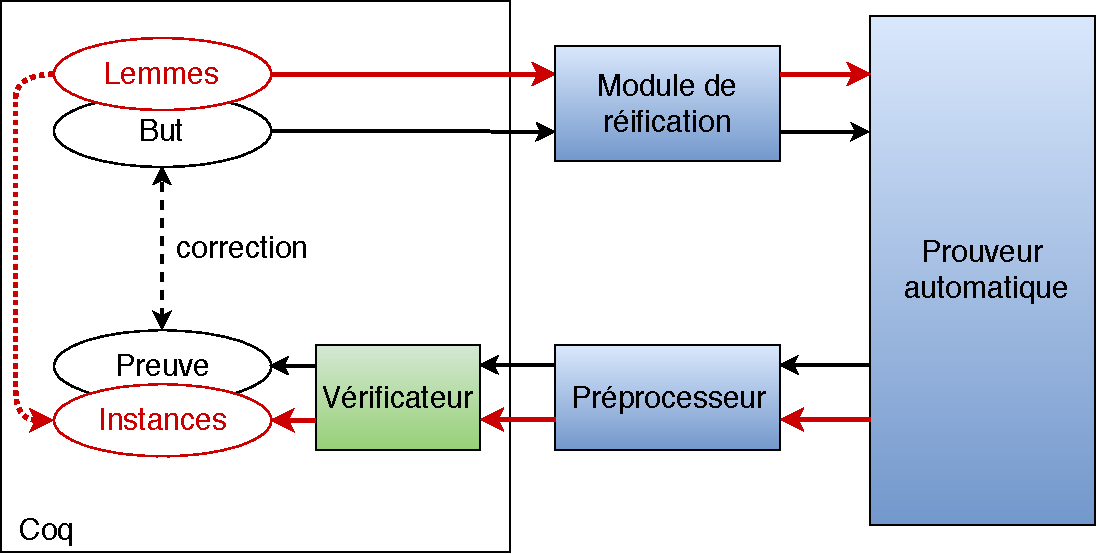
\includegraphics[height=5cm]{ajout_lemmes.pdf}
      \end{center}
    \end{frame}




    \subsection{}
    \begin{frame}{La règle \texttt{ForallInst}}
      \begin{align*}
        &\texttt{Inductive rule :=}\\
        &\texttt{| ... } \\
        &\texttt{| ForallInst }\texttt{(lemma\,:\,Prop) (plemma\,:\,lemma)} \\
        &\texttt{         (inst\,:}\texttt{\,formula) (pinst\,:\,lemma\,->\,interp inst\,=\,true)}
      \end{align*}

      Avantage : le type des formules est inchangé. On utilise la modularité de SMTCoq lors de l'ajout de nouvelles règles.  \\
      \vspace{0.3cm}
      Cas d'application : l'instance ne doit pas contenir de quantificateurs, on se restreint au cas des lemmes en forme prénexe. \\
      \vspace{0.3cm}
      La construction d'une telle règle demande la recherche du lemme correspondant à l'instance.
    \end{frame}




    \subsection{}
    \begin{frame}{Application à veriT : certificats}

      Si le problème n'est pas satisfiable, renvoit un fichier de certificat qui explique pourquoi c'est le cas.

      \hspace{1cm}

      Dans le certificat de veriT suivant, le résultat de la dernière règle est la clause vide $()$ qui représente l'absurde.

      \begin{align*}
        0&:(input\,\,(x \wedge \neg x)) &\texttt{; hypothèse } x \wedge \neg x\\
        1&:(andproj \,\,(\neg x) \,\,0\,\, 2) &\texttt{; de } x \wedge \neg x \texttt{, on obtient } \neg x \\
        2&:(andproj \,\,(x)\,\, 0\,\, 1) &\texttt{; de } x \wedge \neg x \texttt{, on obtient }  x\\
        3&:(resolution \,\,() \,\,2\,\, 1) &\texttt{; de } x \texttt{ et } \neg x \texttt{, on obtient} \perp
      \end{align*}



    \end{frame}


    \begin{frame}{Application à veriT : la règle \texttt{forall\_inst}}

      La règle \texttt{forall\_inst} permet d'instancier les lemmes quantifiés donnés en en entrée dans les certificats de veriT.

      \vspace{1cm}

      Forme générale de l'utilisation de la règle \texttt{forall\_inst} dans les certificats de veriT :
      \begin{align*}
        0&:(input \,\,(\forall x, P \,\, x))) &\texttt{; lemme quantifié} \\
        1&:(forall\_inst \,\,(\neg (\forall x, P \,\, x) \vee (P \, \, c) )) &\texttt{; instanciation} \\
        2&:(resolution  \,\, (P \,\,c) \,\,0 \,\,1) & \text{; instance}
      \end{align*}

    \end{frame}


    \begin{frame}{Application à veriT : traduction de certificats}
      Le préprocesseur transforme les règles
      \begin{flalign*}
        0&:(input \,\,(\forall x, P \,\, x)))&\\
        1&:(forall\_inst \,\,(\neg (\forall x, P \,\, x) \vee (P \, \, c) ))& \\
        2&:(resolution  \,\, (P \,\,c) \,\,0\,\,1)&
      \end{flalign*}
      en :
      \vspace{0.3cm}
      \texttt{ForallInst \_ \_ (P c) \_ } \\
      où les \texttt{\_} sont à compléter (recherche du lemme correspondant, et preuve de l'instanciation). \\
      \vspace{0.3cm}
      $\Longrightarrow$ Suppression de la forme logique de l'implication et des quantificateurs.

      \vspace{5mm}

      Dans l'exemple, la règle de résolution devient redondante.

    \end{frame}


    \begin{frame}{Application à veriT : autres difficultés rencontrées}

      \textit{Parsing} : il faut reconnaître les quantificateurs, problème des variables liées.
      \[ \forall x, (f \,\,(x+1) = f\,\, x \wedge f\,\, 0 = 0)\]

      Reconnaître à quel lemme correspond une instance et montrer que le lemme reconnu implique l'instance.

      \begin{center}
        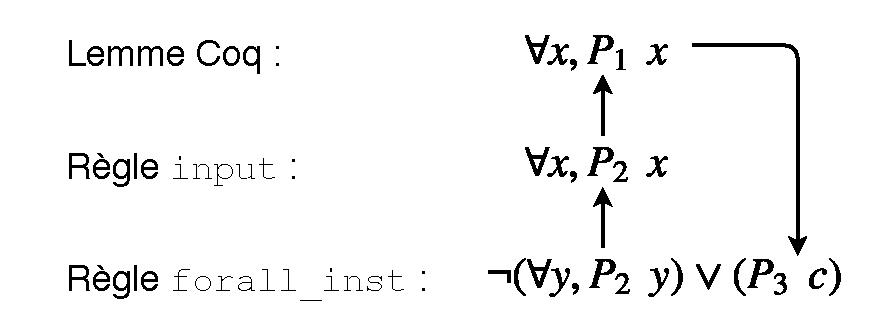
\includegraphics[height=3cm]{other_work_init.pdf}
      \end{center}




    \end{frame}
    \subsection{}
    \begin{frame}{Implémentation}

      La commande \texttt{Add\_lemmas} ajoute les lemmes donnés en argument au contexte. Si aucun lemme n'est donné, la tactique \texttt{verit} garde le même fonctionnement que dans la version initiale de SMTCoq.

      \vspace{3mm}
      Un exemple en Coq :

      \begin{center}
        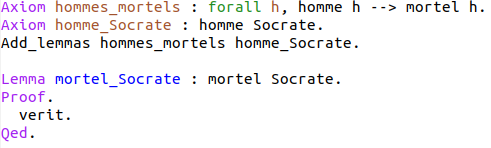
\includegraphics[height=2.5cm]{socrate.png}
      \end{center}
      \vspace{3mm}

      $\longrightarrow $ \texttt{github.com/smtcoq/smtcoq}


    \end{frame}

    \subsection{}
    \begin{frame}{Conclusion}
      Résultats : amélioration de l'expressivité de SMTCoq confirmée par des tests en théorie des groupes, sur une théorie formalisant les listes d'entiers ...

      \vspace{5mm}

      D'autres extensions sont possibles pour étendre les cas d'application de SMTCoq :

      \begin{itemize}
      \item formules dans le type des propositions de Coq
      \item logique du premier ordre
      \end{itemize}

      \vspace{5mm}

      Objectif : faciliter et généraliser l'utilisation de SMTCoq dans les projets développés en Coq.

    \end{frame}


    \end{document}

























    
